\section{Processing and storage of data}
\label{sec:data}

Reconstructed detector events are typically complex data objects described by many parameters. The size of events presents a storage challenge as it can become infeasible to write all reconstructed data to storage at the output rate of the high-level trigger. To overcome this challenge, two key strategies are employed to reduce the size of the reconstructed objects. Firstly, the amount of information can be reduced, by storing only the minimal amount of observables necessary to sufficiently describe the event. Secondly, the object information itself can be compressed, maintaining most or all of the original information while significantly reducing the size of the data being written.

% Streaming
%\subsubsection{Data scouting at ATLAS (TLA) and CMS}
An example of the first approach is the CMS data scouting stream (TLA in ATLAS and Turbo stream in LHCb), wherein events are stored at higher rates with smaller event content - storing simply the online objects, bypassing offline reconstruction entirely. In addition, a parking stream or delayed stream saves event data without running offline reconstruction algorithms, with the intent of processing said events during shutdown periods when computing resources are less constrained. Monitoring and calibration streams are also able to make use of their small event size to store more events, with a typical calibration stream event size of ${\sim}\SI{1.5}{\kilo\byte}$, in comparison to an event with full detector readout at around \SI{2}{\mega\byte}~\cite{cms2023development}. However, the additional information of the latter event model allows a wide range of track reconstruction algorithms to be applied for the identification of $b$-jets, lepton isolation and the mitigation of pile-up vertices~\cite{mia2014trackingcms,tosi2016trackingcms}. 

\begin{figure}[h!]
    \centering
    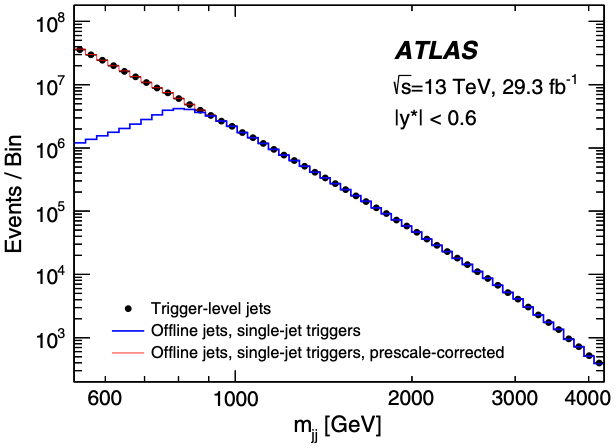
\includegraphics[width=0.55\linewidth]{images/atlas/ATLAS-TLA.png}
    \caption{Comparison of offline and trigger-level jet objects in ATLAS dijet spectra from Ref.~\cite{ATLAS:2018qto}. Trigger-level jets provide low $m_{jj}$ coverage without a requirement for a prescale correction.}
    \label{fig:trigger-level-efficiencies}
\end{figure}

%\subsubsection{The LHCb Turbo model}
Another example of such an approach is the LHCb Turbo model, a reduced-persistency event model, in which only the objects relevant to an HLT2 trigger decision are persisted and saved to a dedicated stream~\cite{Aaij:2016rxn}. For inclusive triggers, which select events across many signals, many objects are still required. To circumvent this, inclusive trigger events are saved to a FULL stream, which can later be reselected by dedicated exclusive lines to extract only the relevant event objects. Many trigger-level objects may be required which are beyond the standard objects of a given decay, for example for flavour tagging. In such cases, selective persistency is applied, whereby an event is saved in the Turbo model with specified additional information, e.g., other tracks arising from a primary vertex, objects contained in a cone around the candidate, etc., A calibration stream (TurCaL) is a special use case of the selective persistence model, wherein only events dedicated to detector alignment and calibration are persisted~\cite{Aaij:2019uij}. % Discuss alignment further <- <- <-


%% COMPRESSION
% Baler? GPUs in ALICE, ML in CMS. Retina?

\subsection{High-level selections}
%ATLAS/CMS, LHCB, ALICE

High-level selection of events and event objects form a core part of trigger implementation. Such selections must be signal efficient, whilst also making decisions sufficiently at a sufficient rate to process the information passed from the detector readout or a low-level trigger. Selection strategies differ between experiments and depend heavily upon detector design, trigger level and physics goals. Selections can be divided into several categories, primary selections corresponding to the main part of physics program, calibration/technical selections used for luminosity determination, alignment \& calibration, monitoring and background estimates and alternative selections which might use experimental implementations. The selection strategies employed by LHC experiments are briefly summarised below.

ATLAS employs a trigger \say{menu}, comprising many trigger chains\footnote{Selection algorithms go by many names: \say{trigger chains} at ATLAS, \say{} at CMS, \say{trigger lines} at LHC.

CMS


The selections at LHCb are generally inclusive for HLT1 and exclusive for HLT2, with further selections applied offline in a process known as sprucing. The main selection of HLT1 is dominated by the one/two-track displaced inclusive trigger. A large fraction of the HLT1 output is also generated by various muon triggers: displaced muon/dimuon, high-mass dimuon and high transverse momentum muon. Unlike HLT1, HLT2 is made up of $\mathcal{O}(1000)$ trigger lines (selection algorithms) tuned for specific analyses. At HLT2, events are either selected exclusively (for which most events are saved in the Turbo event model) or inclusively with a number of triggers, e.g., the topological $b$-trigger~\cite{LHCb:topo-trigger}. Inclusively selected events are persisted in full and further selected offline by exclusive sprucing lines~\cite{LHCb:sprucing}. Dedicated selections for calibration and monitoring are also applied in parallel to selections for physics analysis.


%model follows that for the fixed bandwidth, 10 GB/s due to offline storage resource constrains, the event rate can be increased, and therefore the physics sensitivity of the experiment, by reducing the event size saving only the ``interesting” part of the event. 
